\section{Soorten netwerken}

\textit{In dit hoofdstuk wordt de vraag ``Welke soorten gedistribueerde netwerken worden er gebruikt?'' behandeld. Het doel van de vraag is om de architectuurkeuzes op het gebied van het Distributed Network onderdeel op te stellen, en waar mogelijk is de implicaties van de keuze tegenover het Identity Management onderdeel.}

% In het vooronderzoek is er gevonden dat het consensusproces van grote invloed kan zijn op de architectuurkeuzes van het gedistribueerd netwerk. Er is dan ook voor gekozen om in het onderzoek het netwerksoort synoniem te stellen aan het type consensus die de implementatie gebruikt.

\subsection{Aanpak}

\begin{wrapfigure}[14]{r}{0.5\textwidth}
  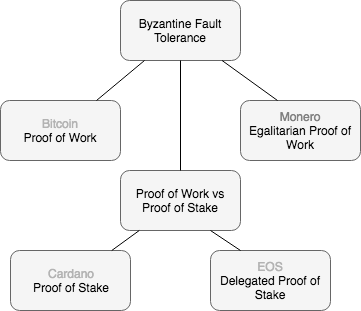
\includegraphics[width=0.5\textwidth]{figures/uitwerking_soorten}
  \caption[Opbouw beantwoording ``Soorten netwerken'']{Termen die als leidraad gebruikt zijn om het resultaat te beschrijven}
  \label{opbouw:netwerken}
\end{wrapfigure}

In fig. \ref{opbouw:netwerken} is te zien welke (globale) termen er gebruikt zijn om de benodigde informatie te vinden. In de meeste gevallen is de beschikbare whitepaper van de implementatie voldoende geweest om de werking van het consensus te beschrijven. Hieronder is de werkwijze en denkwijze uitgeschreven per individueel onderdeel.

\subsubsection{Byzantine Fault Tolerance}
Om deze vraag te beantwoorden is allereerst gezocht naar achtergrondinformatie over consensus en wat het doel ervan is. In het vooronderzoek is er informatie gevonden over het Byzantine Generals Problem \citep{lamport1982byzantine}, waarin, vertaald naar de IT-wereld, wordt gesteld dat het essentieel is voor een betrouwbaar computersysteem om te gaan met fouten in de componenten, waardoor het kan voorkomen dat er conflicterende informatie verstuurd wordt naar de andere componenten van het systeem. 

\subsubsection{Proof of Work}
Hierna zijn bij de implementaties de manier waarop consensus behaald wordt onderzocht. Voor het beschrijven van het Proof of Work algoritme is er gebruik gemaakt van de originele presentatie van het Bitcoin protocol door \cite{nakamoto2008bitcoin}, hierin was alle informatie te vinden die benodigd was. Het egalitarian Proof of Work zoals in gebruik bij Monero is beschreven in \cite{van2013cryptonote} waarin de verschillen en tekortkomingen van het Proof of Work zoals in gebruik bij Bitcoin uiteengezet wordt.

\newpage
\subsubsection{Proof of Stake}
Om een indicatie te geven van de grootste tekortkomingen op het gebied van Proof of Work en redenenen waarom Blockchain implementaties kiezen voor het implementeren van Proof of Stake is er gebruik gemaakt van de whitepaper van Cardano \cite{kiayias2017ouroboros}, waarin de gemotiveerd wordt waarom er voor Proof of Stake is gekozen in plaats van Proof of Work. Naar aanleiding van de primaire reden, namelijk dat Proof of Work enorm veel stroom verspilt, is er gezocht naar een studie die deze claim kan bevestigen, waarbij de studie van \cite{ODwyer:Bitcoin} gebruikt is om dit te bevestigen.

Bij het beschrijven van Delegated Proof of Stake zoals in gebruik bij EOS, bleek de whitepaper niet voldoende informatie te bevatten om het functioneel te beschrijven. Hiervoor is er dan ook een artikel gebruikt dat geschreven is door \cite{steemit:eos_dpos}, waarin het algoritme uitgelegd wordt.

\subsection{Conclusie}

Een gedistribueerd netwerk binnen Blockchain is getypeerd aan het consensus protocol dat gebruikt wordt. In het onderzoek zijn er twee primaire soorten geïdentificeerd, netwerken die gebruik maken van Proof of Stake of van Proof of Work, waarbij Proof of Work gebruik maakt van de rekenkracht van een \gls{node} en Proof of Stake gebruik maakt van de \gls{stake} van een \gls{node}.